\section{Introduzione}\label{sec:introduzione}
\subsection{Pendolo invertito}\label{subsec:intro-pendolo}
Il pendolo invertito su rotaia è un sistema che si presta molto bene ad essere trattato nell'ambito della Teoria del
Controllo.
Il problema che ci poniamo è il seguente:
\begin{framed}
\emph{
    Un pendolo è posto su un carrello libero di muoversi orizzontalmente su una rotaia.
    Il carrello è dotato di un motore che gli permette di accelerare. Conoscendo lo stato del sistema
    $\mathbf x$, trovare un espressione per la forza che deve essere esercitata dal motore $f = f(\mathbf x)$
    che faccia sì che il pendolo si orienti verso l'alto.
  }
\end{framed}
Sebbene sia possibile risolvere questo problema per qualsiasi condizione iniziale del sistema, io tratterò solo il
caso in cui il pendolo parte già in prossimità della posizione verticale. Strategie di \emph{swing-up} e
\emph{swing-down} non saranno oggetto del mio studio.

\subsection{Controller \textsc{LQR}}\label{subsec:intro-lqr}
In generale, nello studio del controllo di un sistema, dobbiamo tenere a mente che la forzante
$\mathbf u$\footnote{La forzante è una matrice, in forma generale. Nel nostro caso, si riduce allo scalare $f$.}
che agisce su di esso, ha un certo costo associato.
Questo è da intendersi sia come costo \emph{materiale} (i.e. il costo della corrente per mettere in moto
un motore) ma, soprattutto, anche come costo \emph{fisico} (i.e. non si può realizzare un motore che ha potenza
infinita).

Un controller \textsc{lqr}, schematizzato in figura \ref{fig:lqr}, permette di risolvere questo problema in modo \emph{ottimale}.
Per spiegare cosa si intende con \emph{ottimale}, citerò direttamente la definizione di \textsc{lqr}:

\begin{framed}
  \textbf{DEF}
  Un controller \textsc{lqr} è una legge di controllo con input $\mathbf x$ e output $\mathbf u$\ldots
  \begin{equation}
    \begin{aligned}[c]
      \mathbf u = -K \mathbf x
    \end{aligned}
    \label{eq:lqr}
  \end{equation}
  \ldots dove la matrice $K$ è costruita in modo tale da minimizzare la seguente funzione costo:
  \begin{equation}
    J(t) \doteq
      \int_0^{+\infty} \left[ \mathbf{x} (s)^* Q \mathbf {x} (s) + \mathbf {u} (s)^* R \mathbf {u} (s) \right] ds
    \label{eq:lqr-costo}
  \end{equation}
  $Q$ ed $R$ sono matrici semidefinite positive che rappresentano, rispettivamente, il costo associato alla
  deviazione dello stato del sistema da $0$ e il costo dell'attuazione del controllo.
\end{framed}

\begin{figure}[h]
  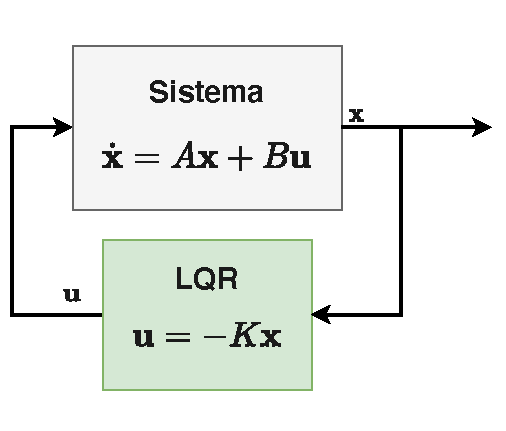
\includegraphics[width=0.5\textwidth]{../assets/diagramma lqr.pdf}
  \caption{\emph{Controller \textsc{lqr}. Lo stato del sistema $\bf x$ è usato dal controller per decidere quale forzante
  $\bf u$ applicare, in modo da ottenere controllo ottimale.}}
  \label{fig:lqr}
\end{figure}

Per poter realizzare un controller di questo tipo, è necessario che il sistema in questione sia \emph{controllabile}.
Darò qualche nozione in più circa la controllabilità nella sezione \ref{subsec:controllabilità}, senza però entrare
troppo nel dettaglio.
Inoltre, ci tengo a precisare che sebbene le equazioni \eqref{eq:lqr} e \eqref{eq:lqr-costo}
valgano per sistemi dinamici a \emph{tempo continuo}, si possono generalizzare tranquillamente a sistemi
a \emph{tempo discreto}.
Rimando a Brunton\cite{brunton2019data} per approfondimenti.

\subsection{Controller \textsc{pid}}\label{subsec:intro-pid}
Un controller \textsc{pid} è un meccanismo di controllo in cui la forzante $\bf u$ è proporzionale a una funzione
errore $e(t)$, definita come differenza tra stato osservato $y(t)$ e stato desiderato $r(t)$ (figura \ref{fig:pid}).

\begin{framed}
  \textbf{DEF}
  Un controller \textsc{pid} è una legge di controllo definita come:
  \begin{equation}
    \begin{aligned}[c]
      u(t) = K_p e(t) + K_d \dot e(t) + K_i \int_0^t e(s)\ ds
    \end{aligned}
    \label{eq:pid}
  \end{equation}
  $K_p$, $K_d$ e $K_i$ sono coefficienti reali positivi.
\end{framed}


\begin{figure}[h]
  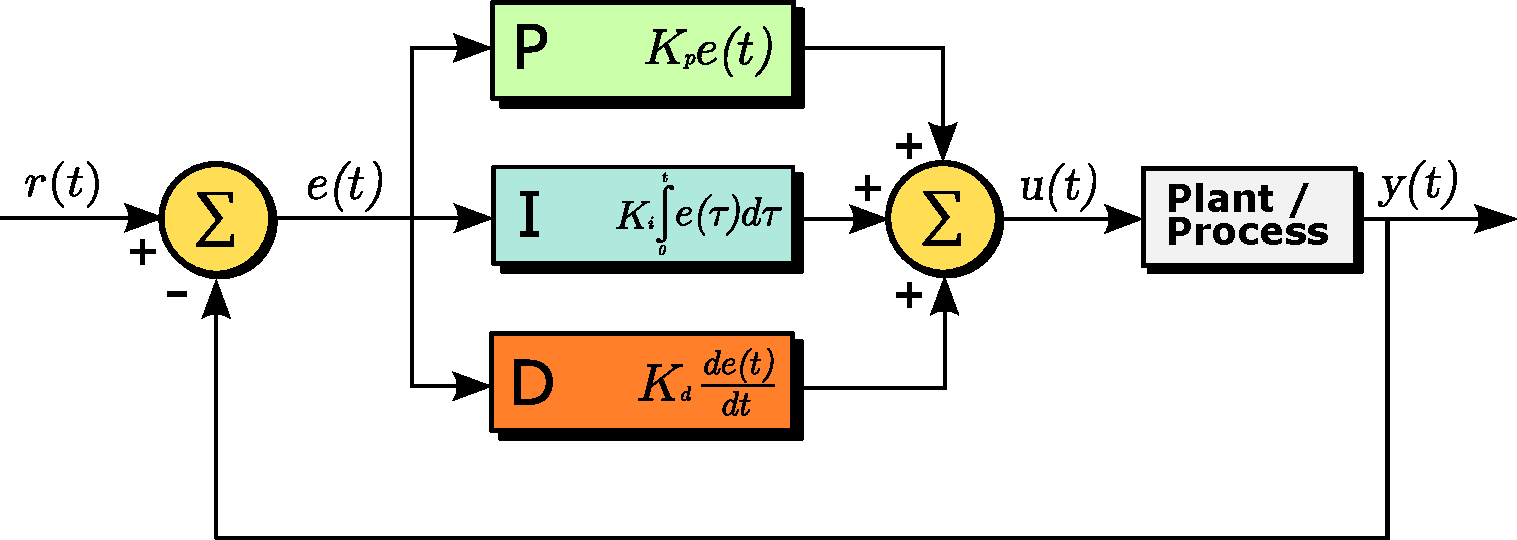
\includegraphics[width=0.5\textwidth]{../assets/diagramma pid.pdf}
  \caption{\emph{Controller \textsc{pid}. $r(t)$ è lo stato desiderato, $y(t)$ è lo stato misurato.}}
  \label{fig:pid}
\end{figure}

Un controller di questo tipo non gode dello stesso background matematico di un controller del tipo \eqref{eq:lqr}.
Il suo vantaggio sta nel fatto che per realizzarlo non è necessaria alcuna conoscenza a priori del modello del sistema.
